\chapter{Merkkijonoalgoritmit}

\index{merkkijono}
\index{aakkosto}

Merkkijonon $s$ merkit ovat $s[1],s[2],\ldots,s[n]$,
missä $n$ on merkkijonon pituus.
\key{Aakkosto} on joukko,
joka määrittää, mitä merkkejä merkkijonossa voi esiintyä.
Esimerkiksi aakkosto $\{\texttt{A},\texttt{B},\ldots,\texttt{Z}\}$
sisältää englannin kielen suuret kirjaimet.

\index{osajono}

\key{Osajono}
sisältää merkkijonon merkit
yhtenäiseltä väliltä.
Merkkijonon osajonojen määrä on $n(n+1)/2$.
Esimerkiksi merkkijonon \texttt{ALGORITMI}
yksi osajono on \texttt{ORITM},
joka muodostuu valitsemalla välin \texttt{ALG\underline{ORITM}I}.

\index{alijono}

\key{Alijono}
on osajoukko merkkijonon merkeistä.
Merkkijonon alijonojen määrä on $2^n-1$.
Esimerkiksi merkkijonon \texttt{ALGORITMI}
yksi alijono on \texttt{LGRMI}, joka muodostuu
valitsemalla merkit \texttt{A\underline{LG}O\underline{R}IT\underline{MI}}.

\index{alkuosa}
\index{loppuosa}
\index{prefiksi}
\index{suffiksi}

\key{Alkuosa} on merkkijonon
alusta alkava osajono,
ja \key{loppuosa} on merkkijonon
loppuun päättyvä osajono.
Esimerkiksi merkkijonon \texttt{KISSA}
alkuosat ovat \texttt{K}, \texttt{KI},
\texttt{KIS}, \texttt{KISS} ja \texttt{KISSA}
ja loppuosat ovat \texttt{A}, \texttt{SA},
\texttt{SSA}, \texttt{ISSA} ja \texttt{KISSA}.
Alkuosa tai loppuosa on \key{aito},
jos se ei ole koko merkkijono.

\index{kierto}

\key{Kierto} syntyy
siirtämällä jokin alkuosa merkkijonon loppuun
tai jokin loppuosa merkkijonon alkuun.
Esimerkiksi merkkijonon \texttt{APILA}
kierrot ovat
\texttt{APILA},
\texttt{PILAA},
\texttt{ILAAP},
\texttt{LAAPI} ja
\texttt{AAPIL}.

\index{jakso}

\key{Jakso} on alkuosa,
jota toistamalla merkkijono muodostuu.
Jakson viimeinen toistokerta voi olla osittainen
niin, että siinä on vain jakson alkuosa.
Usein on kiinnostavaa selvittää, mikä on merkkijonon
\key{lyhin jakso}.
Esimerkiksi merkkijonon \texttt{ABCABCA} lyhin jakso on \texttt{ABC}.
Tässä tapauksessa merkkijono syntyy toistamalla jaksoa ensin kahdesti kokonaan
ja sitten kerran osittain.

\key{Reuna} on
merkkijono, joka on sekä
alkuosa että loppuosa.
Esimerkiksi merkkijonon \texttt{ABADABA}
reunat ovat \texttt{A}, \texttt{ABA} ja
\texttt{ABADABA}.
Usein halutaan etsiä \key{pisin reuna},
joka ei ole koko merkkijono.

\index{leksikografinen järjestys}

Merkkijonojen vertailussa käytössä on yleensä
\key{leksikografinen järjestys}, joka vastaa aakkosjärjestystä.
Siinä $x<y$, jos joko $x$ on $y$:n aito alkuosa
tai on olemassa kohta $k$ niin,
että $x[i]=y[i]$, kun $i<k$, ja $x[k]<y[k]$.

\section{Trie-rakenne}

\index{trie}

\key{Trie} on puurakenne,
joka pitää yllä joukkoa merkkijonoja.
Merkkijonot tallennetaan puuhun
juuresta lähtevinä merkkien ketjuina.
Jos useammalla merkkijonolla on sama alkuosa,
niiden ketjun alkuosa on yhteinen.

Esimerkiksi joukkoa
$\{\texttt{APILA},\texttt{APINA},\texttt{SUU},\texttt{SUURI}\}$
vastaa seuraava trie:

\begin{center}
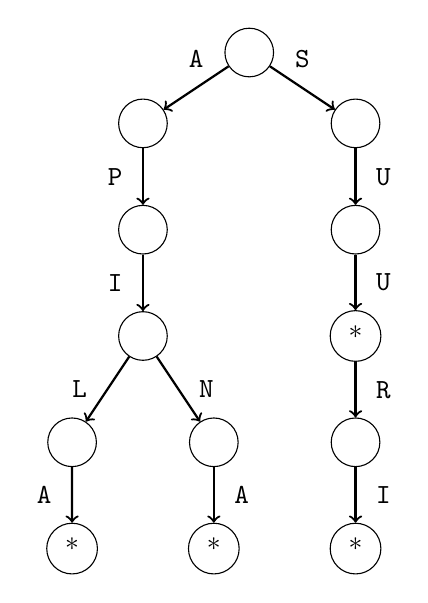
\begin{tikzpicture}[scale=0.9]
\node[draw, circle] (1) at (0,20) {$\phantom{1}$};
\node[draw, circle] (2) at (-1.5,19) {$\phantom{1}$};
\node[draw, circle] (3) at (1.5,19) {$\phantom{1}$};
\node[draw, circle] (4) at (-1.5,17.5) {$\phantom{1}$};
\node[draw, circle] (5) at (-1.5,16) {$\phantom{1}$};
\node[draw, circle] (6) at (-2.5,14.5) {$\phantom{1}$};
\node[draw, circle] (7) at (-0.5,14.5) {$\phantom{1}$};
\node[draw, circle] (8) at (-2.5,13) {*};
\node[draw, circle] (9) at (-0.5,13) {*};
\node[draw, circle] (10) at (1.5,17.5) {$\phantom{1}$};
\node[draw, circle] (11) at (1.5,16) {*};
\node[draw, circle] (12) at (1.5,14.5) {$\phantom{1}$};
\node[draw, circle] (13) at (1.5,13) {*};

\path[draw,thick,->] (1) -- node[font=\small,label=\texttt{A}] {} (2);
\path[draw,thick,->] (1) -- node[font=\small,label=\texttt{S}] {} (3);
\path[draw,thick,->] (2) -- node[font=\small,label=left:\texttt{P}] {} (4);
\path[draw,thick,->] (4) -- node[font=\small,label=left:\texttt{I}] {} (5);
\path[draw,thick,->] (5) -- node[font=\small,label=left:\texttt{L}] {} (6);
\path[draw,thick,->] (5) -- node[font=\small,label=right:\texttt{N}] {} (7);
\path[draw,thick,->] (6) -- node[font=\small,label=left:\texttt{A}] {}(8);
\path[draw,thick,->] (7) -- node[font=\small,label=right:\texttt{A}] {} (9);
\path[draw,thick,->] (3) -- node[font=\small,label=right:\texttt{U}] {} (10);
\path[draw,thick,->] (10) -- node[font=\small,label=right:\texttt{U}] {} (11);
\path[draw,thick,->] (11) -- node[font=\small,label=right:\texttt{R}] {} (12);
\path[draw,thick,->] (12) -- node[font=\small,label=right:\texttt{I}] {} (13);
\end{tikzpicture}
\end{center}
Merkki * solmussa tarkoittaa,
että jokin merkkijono päättyy kyseiseen solmuun.
Tämä merkki on tarpeen,
koska merkkijono voi olla toisen merkkijonon alkuosa,
kuten tässä puussa merkkijonot \texttt{SUU} ja \texttt{SUURI}.

Triessä merkkijono lisääminen ja hakeminen
vievät aikaa $O(n)$, kun $n$ on merkkijonon pituus.
Molemmat operaatiot voi toteuttaa lähtemällä liikkeelle juuresta
ja kulkemalla alaspäin ketjua merkkien mukaisesti.
Tarvittaessa puuhun lisätään uusia solmuja.

Triestä on mahdollista etsiä
sekä merkkijonoja että merkkijonojen alkuosia.
Lisäksi puun solmuissa voi pitää kirjaa,
monessako merkkijonossa on solmua vastaava alkuosa,
mikä lisää trien käyttömahdollisuuksia.

Trie on kätevää tallentaa taulukkona
\begin{lstlisting}
int t[N][A];
\end{lstlisting}
missä $N$ on solmujen suurin mahdollinen määrä
(eli tallennettavien merkkijonojen yhteispituus)
ja $A$ on aakkoston koko.
Ideana on numeroida solmut $1,2,3,\ldots$ niin,
että juuren numero on 1.
Nyt $\texttt{t}[s][c]$ kertoo,
mihin solmuun solmusta $s$ pääsee merkillä $c$.

\section{Merkkijonohajautus}

\index{hajautus}
\index{merkkijonohajautus}

\key{Merkkijonohajautus}
on tekniikka, jonka avulla voi esikäsittelyn
jälkeen tarkistaa tehokkaasti, ovatko
kaksi merkkijonoa samat.
Ideana on verrata toisiinsa merkkijonojen hajautusarvoja,
mikä on tehokkaampaa kuin merkkijonojen
vertaaminen merkki kerrallaan.

\subsubsection*{Hajautusarvon laskeminen}

\index{hajautusarvo}
\index{polynominen hajautus}

Merkkijonon \key{hajautusarvo}
on luku, joka lasketaan merkkijonon merkeistä
etukäteen valitulla tavalla.
Jos kaksi merkkijonoa ovat samat,
myös niiden hajautusarvot ovat samat,
minkä ansiosta merkkijonoja voi vertailla
niiden hajautusarvojen kautta.

Tavallinen tapa toteuttaa merkkijonohajautus
on käyttää polynomista hajautusta.
Siinä hajautusarvo lasketaan kaavalla

\[(c[1] A^{n-1} + c[2] A^{n-2} + \cdots + c[n] A^0) \bmod B  ,\]

missä merkkijonon merkkien koodit ovat
$c[1],c[2],\ldots,c[n]$ ja $A$ ja $B$ ovat etukäteen
valitut vakiot.

Esimerkiksi merkkijonon \texttt{KISSA} merkkien koodit ovat:
\begin{center}
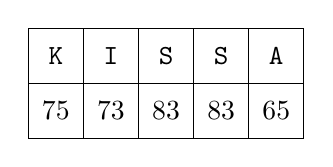
\begin{tikzpicture}[scale=0.7]
\draw (0,0) grid (5,2);

\node at (0.5, 1.5) {\texttt{K}};
\node at (1.5, 1.5) {\texttt{I}};
\node at (2.5, 1.5) {\texttt{S}};
\node at (3.5, 1.5) {\texttt{S}};
\node at (4.5, 1.5) {\texttt{A}};

\node at (0.5, 0.5) {75};
\node at (1.5, 0.5) {73};
\node at (2.5, 0.5) {83};
\node at (3.5, 0.5) {83};
\node at (4.5, 0.5) {65};

\end{tikzpicture}
\end{center}

Jos $A=3$ ja $B=97$, merkkijonon \texttt{KISSA} hajautusarvoksi tulee

\[(75 \cdot 3^4 + 73 \cdot 3^3 + 83 \cdot 3^2 + 83 \cdot 3^1 + 65 \cdot 3^0) \bmod 97 = 59.\]

\subsubsection*{Esikäsittely}

Merkkijonohajautuksen esikäsittely
muodostaa tietoa, jonka avulla 
voi laskea tehokkaasti merkkijonon
osajonojen hajautusarvoja.
Osoittautuu, että polynomisessa hajautuksessa
$O(n)$-aikaisen esikäsittelyn jälkeen voi laskea
minkä tahansa osajonon hajautusarvon
ajassa $O(1)$.

Ideana on muodostaa taulukko $h$,
jossa $h[k]$ on hajautusarvo merkkijonon
alkuosalle kohtaan $k$ asti.
Taulukon voi muodostaa rekursiolla seuraavasti:
\[
\begin{array}{lcl}
h[0] & = & 0 \\
h[k] & = & (h[k-1] A + c[k]) \bmod B \\
\end{array}
\]
Lisäksi muodostetaan taulukko $p$,
jossa $p[k]=A^k \bmod B$:
\[
\begin{array}{lcl}
p[0] & = & 1 \\
p[k] & = & (p[k-1] A) \bmod B. \\
\end{array}
\]
Näiden taulukoiden muodostaminen vie aikaa $O(n)$.
Tämän jälkeen hajautusarvo merkkijonon osajonolle,
joka alkaa kohdasta $a$ ja päättyy kohtaan $b$,
voidaan laskea $O(1)$-ajassa kaavalla
\[(h[b]-h[a-1] p[b-a+1]) \bmod B.\]

\subsubsection*{Hajautuksen käyttö}

Hajautusarvot tarjoavat nopean tavan merkkijonojen
vertailuun.
Ideana on vertailla merkkijonojen koko sisällön
sijasta niiden hajautusarvoja.
Jos hajautusarvot ovat samat,
myös merkkijonot ovat \textit{todennäköisesti} samat,
ja jos taas hajautusarvot eivät ole samat,
merkkijonot eivät ole samat.

Hajautuksen avulla pystyy usein tehostamaan
raa'an voiman algoritmia niin, että siitä tulee
tehokas. Näin on esimerkiksi seuraavassa tehtävässä:

\begin{task}
Annettuna on merkkijono $a$,
jossa on $n$ merkkiä,
sekä merkkijono $b$,
jossa on $m$ merkkiä.
Tehtäväsi on selvittää, montako kertaa
merkkijono $b$ esiintyy merkkijonon $a$ osajonona.
\end{task}

Raa'an voiman algoritmi tehtävään
on käydä läpi kaikki mahdolliset kohdat,
joissa $b$ voi esiintyä $a$:n osajonona,
ja vertailla jokaisessa kohdassa $a$:n ja $b$:n merkkejä.
Mahdollisia kohtia on $O(n)$ ja kukin vertailu
vie aikaa $O(m)$, joten algoritmin aikavaativuus on $O(nm)$.

Algoritmia on mahdollista tehostaa hajautuksen avulla,
koska algoritmissa vertaillaan merkkijonojen osajonoja.
Hajautusta käyttäen kukin vertailu vie aikaa vain $O(1)$
ja tuloksena on algoritmi, jonka aikavaativuus on $O(n)$.
Tämä on tehokkain mahdollinen algoritmi tehtävään.

Yhdistämällä hajautus ja binäärihaku on mahdollista
vertailla myös osajonojen aakkosjärjestystä.
Tätä voi hyödyntää seuraavassa tehtävässä:

\begin{task}
Annettuna on merkkijono,
jossa on $n$ merkkiä,
sekä kokonaisluku $m$.
Tehtäväsi on etsiä merkkijonon
aakkosjärjestyksessä pienin osajono,
jonka pituus on $m$.
\end{task}

Raa'an voiman algoritmi käy läpi
merkkijonon $m$-pituiset osajonot
ja pitää muistissa pienintä löydettyä osajonoa.
Algoritmin aikavaativuus on $O(nm)$,
koska tarkastettavia osajonoja on $O(n)$ ja jokaisen osajonon kohdalla
tehdään $O(m)$-aikainen vertailu aiempaan osajonoon.

Hajautuksen avulla kahden osajonon
aakkosjärjestyksen voi selvittää logaritmisessa
ajassa etsimällä ensin binäärihaulla,
kuinka pitkä on osajonojen yhteinen alkuosa,
ja vertaamalla sitten alkuosan jälkeistä merkkiä.
Niinpä algoritmin aikavaativuudeksi tulee $O(n \log m)$.

\subsubsection*{Törmäykset ja parametrit}

\index{törmäys}

Ilmeinen riski hajautusarvojen vertailussa
on \key{törmäys}, mikä tarkoittaa, että kahdessa merkkijonossa on
eri sisältö mutta niiden hajautusarvot ovat samat.
Tällöin hajautusarvojen perusteella merkkijonot
näyttävät samalta, vaikka todellisuudessa ne eivät ole samat,
ja algoritmi voi toimia väärin.

Törmäyksen riski on aina olemassa,
koska erilaisia merkkijonoja on enemmän kuin
erilaisia hajautusarvoja.
Riskin saa kuitenkin pieneksi valitsemalla
hajautuksen vakiot $A$ ja $B$ huolellisesti.
Vakioiden valinnassa on kaksi tavoitetta:
hajautusarvojen tulisi
jakautua tasaisesti merkkijonoille
ja
erilaisten hajautusarvojen määrän tulisi
olla riittävän suuri.

Hyvä ratkaisu on valita vakioiksi suuria
satunnaislukuja. Tavallinen tapa on valita vakiot
läheltä lukua $10^9$, esimerkiksi

\[
\begin{array}{lcl}
A & = & 911382323 \\
B & = & 972663749 \\
\end{array}
\]

Tällainen valinta takaa sen,
että hajautusarvot jakautuvat
riittävän tasaisesti välille $0 \ldots B-1$.
Suuruusluokan $10^9$ etuna on,
että \texttt{long long} -tyyppi riittää
hajautusarvojen käsittelyyn koodissa,
koska tulot $AB$ ja $BB$ mahtuvat \texttt{long long} -tyyppiin.
Mutta onko $10^9$ riittävä määrä hajautusarvoja?

Tarkastellaan nyt kolmea hajautuksen käyttötapaa:

\textit{Tapaus 1:} Merkkijonoja $x$ ja $y$ verrataan toisiinsa.
Törmäyksen todennäköisyys on $1/B$ olettaen,
että kaikki hajautusarvot esiintyvät yhtä usein.

\textit{Tapaus 2:} Merkkijonoa $x$ verrataan merkkijonoihin
$y_1,y_2,\ldots,y_n$.
Yhden tai useamman törmäyksen todennäköisyys on

\[1-(1-1/B)^n.\]

\textit{Tapaus 3:} Merkkijonoja $x_1,x_2,\ldots,x_n$
verrataan kaikkia keskenään.
Yhden tai useamman törmäyksen todennäköisyys on
\[ 1 - \frac{B \cdot (B-1) \cdot (B-2) \cdots (B-n+1)}{B^n}.\]

Seuraava taulukko sisältää törmäyksen todennäköisyydet,
kun vakion $B$ arvo vaihtelee ja $n=10^6$:

\begin{center}
\begin{tabular}{rrrr}
vakio $B$ & tapaus 1 & tapaus 2 & tapaus 3 \\
\hline
$10^3$ & $0.001000$ & $1.000000$ & $1.000000$ \\
$10^6$ & $0.000001$ & $0.632121$ & $1.000000$ \\
$10^9$ & $0.000000$ & $0.001000$ & $1.000000$ \\
$10^{12}$ & $0.000000$ & $0.000000$ & $0.393469$ \\
$10^{15}$ & $0.000000$ & $0.000000$ & $0.000500$ \\
$10^{18}$ & $0.000000$ & $0.000000$ & $0.000001$ \\
\end{tabular}
\end{center}

Taulukosta näkee, että tapauksessa 1
törmäyksen riski on olematon
valinnalla $B \approx 10^9$.
Tapauksessa 2 riski on olemassa, mutta se on silti edelleen vähäinen.
Tapauksessa 3 tilanne on kuitenkin täysin toinen:
törmäys tapahtuu käytännössä varmasti
vielä valinnalla $B \approx 10^9$.

\index{syntymäpäiväparadoksi}

Tapauksen 3 ilmiö tunnetaan nimellä
\key{syntymäpäiväparadoksi}:
jos huoneessa on $n$ henkilöä, on suuri
todennäköisyys, että jollain kahdella
henkilöllä on sama syntymäpäivä, vaikka
$n$ olisi melko pieni.
Vastaavasti hajautuksessa kun kaikkia
hajautusarvoja verrataan keskenään,
käy helposti niin, että jotkin
kaksi ovat sattumalta samoja.

Hyvä tapa pienentää törmäyksen riskiä on laskea
\emph{useita} hajautusarvoja eri parametreilla
ja verrata niitä kaikkia.
On hyvin pieni todennäköisyys,
että törmäys tapahtuisi samaan aikaan
kaikissa hajautusarvoissa.
Esimerkiksi kaksi hajautusarvoa parametrilla
$B \approx 10^9$ vastaa yhtä hajautusarvoa
parametrilla $B \approx 10^{18}$,
mikä takaa hyvän suojan törmäyksiltä.

Jotkut käyttävät hajautuksessa vakioita $B=2^{32}$ tai $B=2^{64}$,
jolloin modulo $B$ tulee laskettua
automaattisesti, kun muuttujan arvo pyörähtää ympäri.
Tämä ei ole kuitenkaan hyvä valinta,
koska muotoa $2^x$ olevaa moduloa vastaan
pystyy tekemään testisyötteen, joka aiheuttaa varmasti törmäyksen.

\section{Z-algoritmi}

\index{Z-algoritmi}
\index{Z-taulukko}

\key{Z-algoritmi} muodostaa merkkijonosta \key{Z-taulukon},
joka kertoo kullekin merkkijonon kohdalle,
mikä on pisin kyseisestä kohdasta alkava osajono,
joka on myös merkkijonon alkuosa.
Z-algoritmin avulla voi ratkaista tehokkaasti
monia merkkijonotehtäviä.

Z-algoritmi ja merkkijonohajautus ovat usein
vaihtoehtoisia tekniikoita, ja on makuasia,
kumpaa algoritmia käyttää.
Toisin kuin hajautus, Z-algoritmi toimii
varmasti oikein eikä siinä ole törmäysten riskiä.
Toisaalta Z-algoritmi on vaikeampi toteuttaa eikä
se sovellu kaikkeen samaan kuin hajautus.

\subsubsection*{Algoritmin toiminta}

Z-algoritmi muodostaa merkkijonolle Z-taulukon,
jonka jokaisessa kohdassa lukee,
kuinka pitkälle kohdasta
alkava osajono vastaa merkkijonon alkuosaa.
Esimerkiksi Z-taulukko
merkkijonolle \texttt{ACBACDACBACBACDA} on seuraava:

\begin{center}
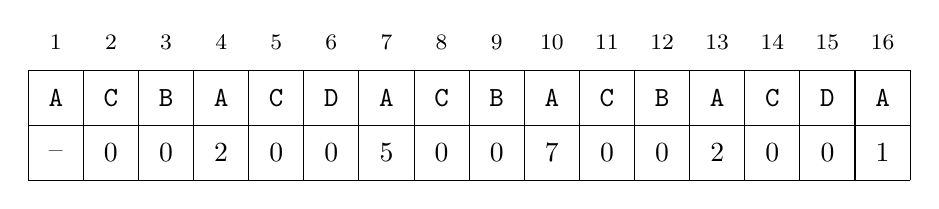
\begin{tikzpicture}[scale=0.7]
\draw (0,0) grid (16,2);

\node at (0.5, 1.5) {\texttt{A}};
\node at (1.5, 1.5) {\texttt{C}};
\node at (2.5, 1.5) {\texttt{B}};
\node at (3.5, 1.5) {\texttt{A}};
\node at (4.5, 1.5) {\texttt{C}};
\node at (5.5, 1.5) {\texttt{D}};
\node at (6.5, 1.5) {\texttt{A}};
\node at (7.5, 1.5) {\texttt{C}};
\node at (8.5, 1.5) {\texttt{B}};
\node at (9.5, 1.5) {\texttt{A}};
\node at (10.5, 1.5) {\texttt{C}};
\node at (11.5, 1.5) {\texttt{B}};
\node at (12.5, 1.5) {\texttt{A}};
\node at (13.5, 1.5) {\texttt{C}};
\node at (14.5, 1.5) {\texttt{D}};
\node at (15.5, 1.5) {\texttt{A}};

\node at (0.5, 0.5) {--};
\node at (1.5, 0.5) {0};
\node at (2.5, 0.5) {0};
\node at (3.5, 0.5) {2};
\node at (4.5, 0.5) {0};
\node at (5.5, 0.5) {0};
\node at (6.5, 0.5) {5};
\node at (7.5, 0.5) {0};
\node at (8.5, 0.5) {0};
\node at (9.5, 0.5) {7};
\node at (10.5, 0.5) {0};
\node at (11.5, 0.5) {0};
\node at (12.5, 0.5) {2};
\node at (13.5, 0.5) {0};
\node at (14.5, 0.5) {0};
\node at (15.5, 0.5) {1};

\footnotesize
\node at (0.5, 2.5) {1};
\node at (1.5, 2.5) {2};
\node at (2.5, 2.5) {3};
\node at (3.5, 2.5) {4};
\node at (4.5, 2.5) {5};
\node at (5.5, 2.5) {6};
\node at (6.5, 2.5) {7};
\node at (7.5, 2.5) {8};
\node at (8.5, 2.5) {9};
\node at (9.5, 2.5) {10};
\node at (10.5, 2.5) {11};
\node at (11.5, 2.5) {12};
\node at (12.5, 2.5) {13};
\node at (13.5, 2.5) {14};
\node at (14.5, 2.5) {15};
\node at (15.5, 2.5) {16};

\end{tikzpicture}
\end{center}

Esimerkiksi kohdassa 7 on arvo 5,
koska siitä alkava 5-merkkinen osajono
\texttt{ACBAC} on merkkijonon alkuosa,
mutta 6-merkkinen osajono \texttt{ACBACB}
ei ole enää merkkijonon alkuosa.

Z-algoritmi käy läpi merkkijonon
vasemmalta oikealle ja laskee
jokaisessa kohdassa,
kuinka pitkälle kyseisestä kohdasta alkava
osajono täsmää merkkijonon alkuun.
Algoritmi laskee yhteisen
alkuosan pituuden vertaamalla
merkkijonon alkua ja osajonon alkua toisiinsa.

Suoraviivaisesti toteutettuna
tällaisen algoritmin aikavaativuus olisi $O(n^2)$,
koska yhteiset alkuosat voivat olla pitkiä.
Z-algoritmissa on kuitenkin yksi tärkeä
optimointi, jonka ansiosta algoritmin
aikavaativuus on vain $O(n)$.

Ideana on pitää muistissa väliä $[x,y]$,
joka on aiemmin laskettu merkkijonon
alkuun täsmäävä väli, jossa $y$ on 
mahdollisimman suuri.
Tällä välillä olevia
merkkejä ei tarvitse koskaan
verrata uudestaan
merkkijonon alkuun, vaan niitä koskevan
tiedon saa suoraan Z-taulukon lasketusta osasta.

Z-algoritmin aikavaativuus on $O(n)$,
koska algoritmi aloittaa merkki kerrallaan
vertailun aina kohdasta $y+1$.
Jos merkit täsmäävät, kohta $y$
siirtyy eteenpäin
eikä algoritmin tarvitse enää
koskaan vertailla tätä kohtaa,
vaan se pystyy hyödyntämään
Z-taulukon alussa olevaa tietoa.

\subsubsection*{Esimerkki}

Katsotaan nyt, miten Z-algoritmi muodostaa
seuraavan Z-taulukon:

\begin{center}
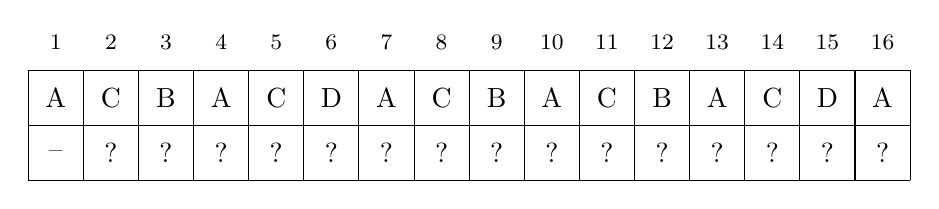
\begin{tikzpicture}[scale=0.7]
\draw (0,0) grid (16,2);

\node at (0.5, 1.5) {A};
\node at (1.5, 1.5) {C};
\node at (2.5, 1.5) {B};
\node at (3.5, 1.5) {A};
\node at (4.5, 1.5) {C};
\node at (5.5, 1.5) {D};
\node at (6.5, 1.5) {A};
\node at (7.5, 1.5) {C};
\node at (8.5, 1.5) {B};
\node at (9.5, 1.5) {A};
\node at (10.5, 1.5) {C};
\node at (11.5, 1.5) {B};
\node at (12.5, 1.5) {A};
\node at (13.5, 1.5) {C};
\node at (14.5, 1.5) {D};
\node at (15.5, 1.5) {A};

\node at (0.5, 0.5) {--};
\node at (1.5, 0.5) {?};
\node at (2.5, 0.5) {?};
\node at (3.5, 0.5) {?};
\node at (4.5, 0.5) {?};
\node at (5.5, 0.5) {?};
\node at (6.5, 0.5) {?};
\node at (7.5, 0.5) {?};
\node at (8.5, 0.5) {?};
\node at (9.5, 0.5) {?};
\node at (10.5, 0.5) {?};
\node at (11.5, 0.5) {?};
\node at (12.5, 0.5) {?};
\node at (13.5, 0.5) {?};
\node at (14.5, 0.5) {?};
\node at (15.5, 0.5) {?};

\footnotesize
\node at (0.5, 2.5) {1};
\node at (1.5, 2.5) {2};
\node at (2.5, 2.5) {3};
\node at (3.5, 2.5) {4};
\node at (4.5, 2.5) {5};
\node at (5.5, 2.5) {6};
\node at (6.5, 2.5) {7};
\node at (7.5, 2.5) {8};
\node at (8.5, 2.5) {9};
\node at (9.5, 2.5) {10};
\node at (10.5, 2.5) {11};
\node at (11.5, 2.5) {12};
\node at (12.5, 2.5) {13};
\node at (13.5, 2.5) {14};
\node at (14.5, 2.5) {15};
\node at (15.5, 2.5) {16};

\end{tikzpicture}
\end{center}

Ensimmäinen mielenkiintoinen kohta tulee,
kun yhteisen alkuosan pituus on 5.
Silloin algoritmi laittaa muistiin
välin $[7,11]$ seuraavasti:

\begin{center}
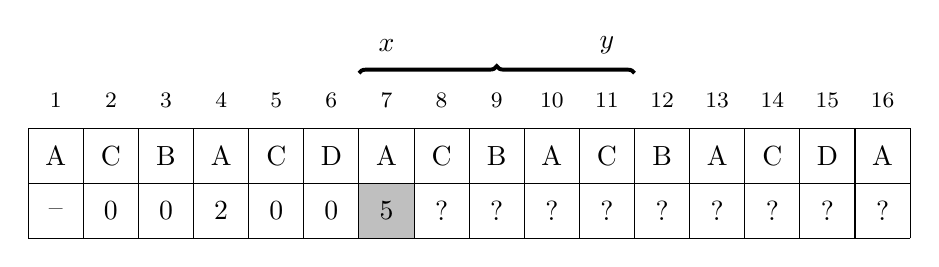
\begin{tikzpicture}[scale=0.7]
\fill[color=lightgray] (6,0) rectangle (7,1);
\draw (0,0) grid (16,2);

\node at (0.5, 1.5) {A};
\node at (1.5, 1.5) {C};
\node at (2.5, 1.5) {B};
\node at (3.5, 1.5) {A};
\node at (4.5, 1.5) {C};
\node at (5.5, 1.5) {D};
\node at (6.5, 1.5) {A};
\node at (7.5, 1.5) {C};
\node at (8.5, 1.5) {B};
\node at (9.5, 1.5) {A};
\node at (10.5, 1.5) {C};
\node at (11.5, 1.5) {B};
\node at (12.5, 1.5) {A};
\node at (13.5, 1.5) {C};
\node at (14.5, 1.5) {D};
\node at (15.5, 1.5) {A};

\node at (0.5, 0.5) {--};
\node at (1.5, 0.5) {0};
\node at (2.5, 0.5) {0};
\node at (3.5, 0.5) {2};
\node at (4.5, 0.5) {0};
\node at (5.5, 0.5) {0};
\node at (6.5, 0.5) {5};
\node at (7.5, 0.5) {?};
\node at (8.5, 0.5) {?};
\node at (9.5, 0.5) {?};
\node at (10.5, 0.5) {?};
\node at (11.5, 0.5) {?};
\node at (12.5, 0.5) {?};
\node at (13.5, 0.5) {?};
\node at (14.5, 0.5) {?};
\node at (15.5, 0.5) {?};

\draw [decoration={brace}, decorate, line width=0.5mm] (6,3.00) -- (11,3.00);

\node at (6.5,3.50) {$x$};
\node at (10.5,3.50) {$y$};


\footnotesize
\node at (0.5, 2.5) {1};
\node at (1.5, 2.5) {2};
\node at (2.5, 2.5) {3};
\node at (3.5, 2.5) {4};
\node at (4.5, 2.5) {5};
\node at (5.5, 2.5) {6};
\node at (6.5, 2.5) {7};
\node at (7.5, 2.5) {8};
\node at (8.5, 2.5) {9};
\node at (9.5, 2.5) {10};
\node at (10.5, 2.5) {11};
\node at (11.5, 2.5) {12};
\node at (12.5, 2.5) {13};
\node at (13.5, 2.5) {14};
\node at (14.5, 2.5) {15};
\node at (15.5, 2.5) {16};

\end{tikzpicture}
\end{center}

Välin $[7,11]$ hyötynä on, että algoritmi
voi sen avulla laskea seuraavat
Z-taulukon arvot nopeammin.
Koska välin $[7,11]$ merkit ovat samat
kuin merkkijonon alussa,
myös Z-taulukon arvoissa on vastaavuutta.

Ensinnäkin kohdissa 8 ja 9
tulee olla samat arvot kuin
kohdissa 2 ja 3,
koska väli $[7,11]$
vastaa väliä $[1,5]$:

\begin{center}
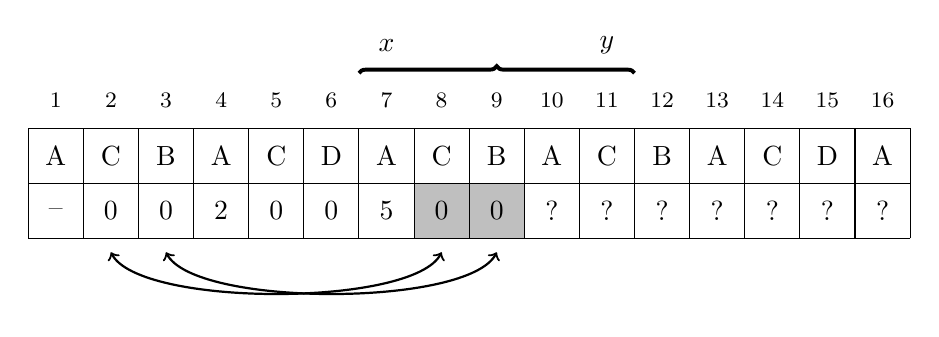
\begin{tikzpicture}[scale=0.7]
\fill[color=lightgray] (7,0) rectangle (9,1);
\draw (0,0) grid (16,2);

\node at (0.5, 1.5) {A};
\node at (1.5, 1.5) {C};
\node at (2.5, 1.5) {B};
\node at (3.5, 1.5) {A};
\node at (4.5, 1.5) {C};
\node at (5.5, 1.5) {D};
\node at (6.5, 1.5) {A};
\node at (7.5, 1.5) {C};
\node at (8.5, 1.5) {B};
\node at (9.5, 1.5) {A};
\node at (10.5, 1.5) {C};
\node at (11.5, 1.5) {B};
\node at (12.5, 1.5) {A};
\node at (13.5, 1.5) {C};
\node at (14.5, 1.5) {D};
\node at (15.5, 1.5) {A};

\node at (0.5, 0.5) {--};
\node at (1.5, 0.5) {0};
\node at (2.5, 0.5) {0};
\node at (3.5, 0.5) {2};
\node at (4.5, 0.5) {0};
\node at (5.5, 0.5) {0};
\node at (6.5, 0.5) {5};
\node at (7.5, 0.5) {0};
\node at (8.5, 0.5) {0};
\node at (9.5, 0.5) {?};
\node at (10.5, 0.5) {?};
\node at (11.5, 0.5) {?};
\node at (12.5, 0.5) {?};
\node at (13.5, 0.5) {?};
\node at (14.5, 0.5) {?};
\node at (15.5, 0.5) {?};


\draw [decoration={brace}, decorate, line width=0.5mm] (6,3.00) -- (11,3.00);

\node at (6.5,3.50) {$x$};
\node at (10.5,3.50) {$y$};


\footnotesize
\node at (0.5, 2.5) {1};
\node at (1.5, 2.5) {2};
\node at (2.5, 2.5) {3};
\node at (3.5, 2.5) {4};
\node at (4.5, 2.5) {5};
\node at (5.5, 2.5) {6};
\node at (6.5, 2.5) {7};
\node at (7.5, 2.5) {8};
\node at (8.5, 2.5) {9};
\node at (9.5, 2.5) {10};
\node at (10.5, 2.5) {11};
\node at (11.5, 2.5) {12};
\node at (12.5, 2.5) {13};
\node at (13.5, 2.5) {14};
\node at (14.5, 2.5) {15};
\node at (15.5, 2.5) {16};


\draw[thick,<->] (7.5,-0.25) .. controls (7,-1.25) and (2,-1.25) .. (1.5,-0.25);
\draw[thick,<->] (8.5,-0.25) .. controls (8,-1.25) and (3,-1.25) .. (2.5,-0.25);
\end{tikzpicture}
\end{center}

Seuraavaksi kohdasta 4 saa tietoa kohdan
10 arvon laskemiseksi.
Koska kohdassa 4 on arvo 2,
tämä tarkoittaa, että osajono
täsmää kohtaan $y=11$ asti,
mutta sen jälkeen on tutkimatonta
aluetta merkkijonossa.

\begin{center}
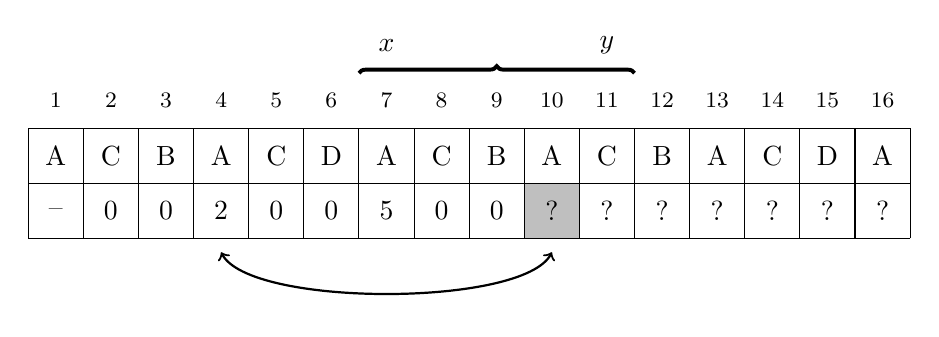
\begin{tikzpicture}[scale=0.7]
\fill[color=lightgray] (9,0) rectangle (10,1);
\draw (0,0) grid (16,2);

\node at (0.5, 1.5) {A};
\node at (1.5, 1.5) {C};
\node at (2.5, 1.5) {B};
\node at (3.5, 1.5) {A};
\node at (4.5, 1.5) {C};
\node at (5.5, 1.5) {D};
\node at (6.5, 1.5) {A};
\node at (7.5, 1.5) {C};
\node at (8.5, 1.5) {B};
\node at (9.5, 1.5) {A};
\node at (10.5, 1.5) {C};
\node at (11.5, 1.5) {B};
\node at (12.5, 1.5) {A};
\node at (13.5, 1.5) {C};
\node at (14.5, 1.5) {D};
\node at (15.5, 1.5) {A};

\node at (0.5, 0.5) {--};
\node at (1.5, 0.5) {0};
\node at (2.5, 0.5) {0};
\node at (3.5, 0.5) {2};
\node at (4.5, 0.5) {0};
\node at (5.5, 0.5) {0};
\node at (6.5, 0.5) {5};
\node at (7.5, 0.5) {0};
\node at (8.5, 0.5) {0};
\node at (9.5, 0.5) {?};
\node at (10.5, 0.5) {?};
\node at (11.5, 0.5) {?};
\node at (12.5, 0.5) {?};
\node at (13.5, 0.5) {?};
\node at (14.5, 0.5) {?};
\node at (15.5, 0.5) {?};

\draw [decoration={brace}, decorate, line width=0.5mm] (6,3.00) -- (11,3.00);

\node at (6.5,3.50) {$x$};
\node at (10.5,3.50) {$y$};


\footnotesize
\node at (0.5, 2.5) {1};
\node at (1.5, 2.5) {2};
\node at (2.5, 2.5) {3};
\node at (3.5, 2.5) {4};
\node at (4.5, 2.5) {5};
\node at (5.5, 2.5) {6};
\node at (6.5, 2.5) {7};
\node at (7.5, 2.5) {8};
\node at (8.5, 2.5) {9};
\node at (9.5, 2.5) {10};
\node at (10.5, 2.5) {11};
\node at (11.5, 2.5) {12};
\node at (12.5, 2.5) {13};
\node at (13.5, 2.5) {14};
\node at (14.5, 2.5) {15};
\node at (15.5, 2.5) {16};

\draw[thick,<->] (9.5,-0.25) .. controls (9,-1.25) and (4,-1.25) .. (3.5,-0.25);
\end{tikzpicture}
\end{center}

Nyt algoritmi alkaa vertailla merkkejä
kohdasta $y+1=12$ alkaen merkki kerrallaan.
Algoritmi ei voi hyödyntää valmiina
Z-taulukossa olevaa tietoa, koska se ei ole vielä aiemmin
tutkinut merkkijonoa näin pitkälle.
Tuloksena osajonon pituudeksi tulee 7
ja väli $[x,y]$ päivittyy vastaavasti:

\begin{center}
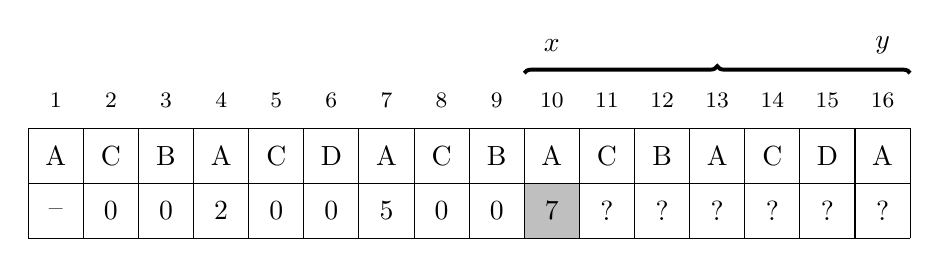
\begin{tikzpicture}[scale=0.7]
\fill[color=lightgray] (9,0) rectangle (10,1);
\draw (0,0) grid (16,2);

\node at (0.5, 1.5) {A};
\node at (1.5, 1.5) {C};
\node at (2.5, 1.5) {B};
\node at (3.5, 1.5) {A};
\node at (4.5, 1.5) {C};
\node at (5.5, 1.5) {D};
\node at (6.5, 1.5) {A};
\node at (7.5, 1.5) {C};
\node at (8.5, 1.5) {B};
\node at (9.5, 1.5) {A};
\node at (10.5, 1.5) {C};
\node at (11.5, 1.5) {B};
\node at (12.5, 1.5) {A};
\node at (13.5, 1.5) {C};
\node at (14.5, 1.5) {D};
\node at (15.5, 1.5) {A};

\node at (0.5, 0.5) {--};
\node at (1.5, 0.5) {0};
\node at (2.5, 0.5) {0};
\node at (3.5, 0.5) {2};
\node at (4.5, 0.5) {0};
\node at (5.5, 0.5) {0};
\node at (6.5, 0.5) {5};
\node at (7.5, 0.5) {0};
\node at (8.5, 0.5) {0};
\node at (9.5, 0.5) {7};
\node at (10.5, 0.5) {?};
\node at (11.5, 0.5) {?};
\node at (12.5, 0.5) {?};
\node at (13.5, 0.5) {?};
\node at (14.5, 0.5) {?};
\node at (15.5, 0.5) {?};

\draw [decoration={brace}, decorate, line width=0.5mm] (9,3.00) -- (16,3.00);

\node at (9.5,3.50) {$x$};
\node at (15.5,3.50) {$y$};


\footnotesize
\node at (0.5, 2.5) {1};
\node at (1.5, 2.5) {2};
\node at (2.5, 2.5) {3};
\node at (3.5, 2.5) {4};
\node at (4.5, 2.5) {5};
\node at (5.5, 2.5) {6};
\node at (6.5, 2.5) {7};
\node at (7.5, 2.5) {8};
\node at (8.5, 2.5) {9};
\node at (9.5, 2.5) {10};
\node at (10.5, 2.5) {11};
\node at (11.5, 2.5) {12};
\node at (12.5, 2.5) {13};
\node at (13.5, 2.5) {14};
\node at (14.5, 2.5) {15};
\node at (15.5, 2.5) {16};

% \draw[thick,<->] (9.5,-0.25) .. controls (9,-1.25) and (4,-1.25) .. (3.5,-0.25);
\end{tikzpicture}
\end{center}

Tämän jälkeen kaikkien seuraavien Z-taulukon
arvojen laskemisessa pystyy hyödyntämään
jälleen välin $[x,y]$ antamaa tietoa
ja algoritmi saa Z-taulukon loppuun tulevat
arvot suoraan Z-taulukon alusta:

\begin{center}
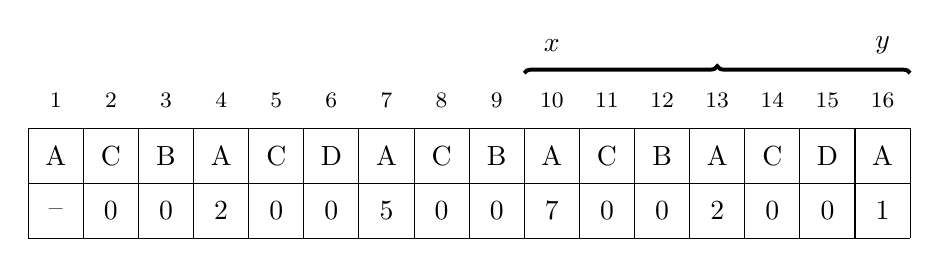
\begin{tikzpicture}[scale=0.7]
\draw (0,0) grid (16,2);

\node at (0.5, 1.5) {A};
\node at (1.5, 1.5) {C};
\node at (2.5, 1.5) {B};
\node at (3.5, 1.5) {A};
\node at (4.5, 1.5) {C};
\node at (5.5, 1.5) {D};
\node at (6.5, 1.5) {A};
\node at (7.5, 1.5) {C};
\node at (8.5, 1.5) {B};
\node at (9.5, 1.5) {A};
\node at (10.5, 1.5) {C};
\node at (11.5, 1.5) {B};
\node at (12.5, 1.5) {A};
\node at (13.5, 1.5) {C};
\node at (14.5, 1.5) {D};
\node at (15.5, 1.5) {A};

\node at (0.5, 0.5) {--};
\node at (1.5, 0.5) {0};
\node at (2.5, 0.5) {0};
\node at (3.5, 0.5) {2};
\node at (4.5, 0.5) {0};
\node at (5.5, 0.5) {0};
\node at (6.5, 0.5) {5};
\node at (7.5, 0.5) {0};
\node at (8.5, 0.5) {0};
\node at (9.5, 0.5) {7};
\node at (10.5, 0.5) {0};
\node at (11.5, 0.5) {0};
\node at (12.5, 0.5) {2};
\node at (13.5, 0.5) {0};
\node at (14.5, 0.5) {0};
\node at (15.5, 0.5) {1};

\draw [decoration={brace}, decorate, line width=0.5mm] (9,3.00) -- (16,3.00);

\node at (9.5,3.50) {$x$};
\node at (15.5,3.50) {$y$};


\footnotesize
\node at (0.5, 2.5) {1};
\node at (1.5, 2.5) {2};
\node at (2.5, 2.5) {3};
\node at (3.5, 2.5) {4};
\node at (4.5, 2.5) {5};
\node at (5.5, 2.5) {6};
\node at (6.5, 2.5) {7};
\node at (7.5, 2.5) {8};
\node at (8.5, 2.5) {9};
\node at (9.5, 2.5) {10};
\node at (10.5, 2.5) {11};
\node at (11.5, 2.5) {12};
\node at (12.5, 2.5) {13};
\node at (13.5, 2.5) {14};
\node at (14.5, 2.5) {15};
\node at (15.5, 2.5) {16};

\end{tikzpicture}
\end{center}

\subsubsection{Z-taulukon käyttö}

Z-taulukon avulla pystyy ratkaisemaan
tehokkaasti monia merkkijonotehtäviä.
Ratkaistaan esimerkkinä seuraava tehtävä:
\begin{task}
Annettuna on merkkijono $a$,
jossa on $n$ merkkiä,
sekä merkkijono $b$,
jossa on $m$ merkkiä.
Tehtäväsi on selvittää, montako kertaa
merkkijono $b$ esiintyy merkkijonon $a$ osajonona.
\end{task}

\noindent
Usein esiintyvä idea Z-algoritmin yhteydessä
on muodostaa merkkijono,
jonka osana on useita välimerkeillä
erotettuja merkkijonoja.
Tässä tehtävässä sopiva merkkijono on
$b$\texttt{\#}$a$,
jossa merkkijonojen $b$ ja $a$ välissä on
erikoismerkki \texttt{\#},
jota ei esiinny merkkijonoissa.

Merkkijonon $b$\texttt{\#}$a$ hyötynä on,
että sitä vastaava Z-taulukko kertoo,
missä kohdissa merkkijonoa $a$
esiintyy merkkijono $b$.
Tällaiset kohdat ovat tarkalleen ne
Z-taulukon kohdat, joissa on luku $m$.
Algoritmin aikavaativuus on $O(n)$,
koska riittää muodostaa Z-taulukko ja käydä se läpi.

\begin{samepage}
Esimerkiksi jos $a=$\texttt{HATTIVATTI} ja $b=$\texttt{ATT},
niin Z-taulukosta tulee:

\begin{center}
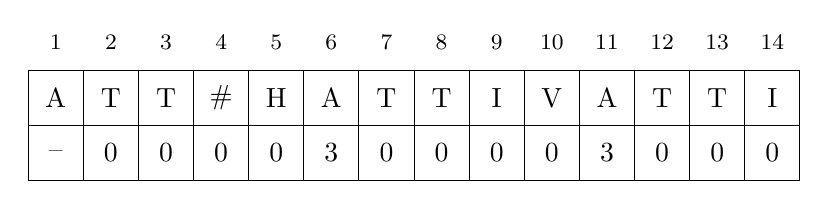
\begin{tikzpicture}[scale=0.7]
\draw (0,0) grid (14,2);

\node at (0.5, 1.5) {A};
\node at (1.5, 1.5) {T};
\node at (2.5, 1.5) {T};
\node at (3.5, 1.5) {\#};
\node at (4.5, 1.5) {H};
\node at (5.5, 1.5) {A};
\node at (6.5, 1.5) {T};
\node at (7.5, 1.5) {T};
\node at (8.5, 1.5) {I};
\node at (9.5, 1.5) {V};
\node at (10.5, 1.5) {A};
\node at (11.5, 1.5) {T};
\node at (12.5, 1.5) {T};
\node at (13.5, 1.5) {I};

\node at (0.5, 0.5) {--};
\node at (1.5, 0.5) {0};
\node at (2.5, 0.5) {0};
\node at (3.5, 0.5) {0};
\node at (4.5, 0.5) {0};
\node at (5.5, 0.5) {3};
\node at (6.5, 0.5) {0};
\node at (7.5, 0.5) {0};
\node at (8.5, 0.5) {0};
\node at (9.5, 0.5) {0};
\node at (10.5, 0.5) {3};
\node at (11.5, 0.5) {0};
\node at (12.5, 0.5) {0};
\node at (13.5, 0.5) {0};

\footnotesize
\node at (0.5, 2.5) {1};
\node at (1.5, 2.5) {2};
\node at (2.5, 2.5) {3};
\node at (3.5, 2.5) {4};
\node at (4.5, 2.5) {5};
\node at (5.5, 2.5) {6};
\node at (6.5, 2.5) {7};
\node at (7.5, 2.5) {8};
\node at (8.5, 2.5) {9};
\node at (9.5, 2.5) {10};
\node at (10.5, 2.5) {11};
\node at (11.5, 2.5) {12};
\node at (12.5, 2.5) {13};
\node at (13.5, 2.5) {14};
\end{tikzpicture}
\end{center}
\end{samepage}

Taulukon kohdissa 6 ja 11 on luku 3,
mikä tarkoittaa, että \texttt{ATT}
esiintyy vastaavissa kohdissa merkkijonossa
\texttt{HATTIVATTI}.

\subsubsection{Algoritmin toteutus}

Seuraavassa on lyhyt Z-algoritmin toteutus,
joka palauttaa Z-taulukon vektorina.
Huomaa, että tässä toteutuksessa merkkijonossa
ja taulukossa on 0-indeksointi
toisin kuin yllä olevissa esimerkeissä.

\begin{lstlisting}
vector<int> z(string s) {
    int n = s.size();
    vector<int> z(n);
    int x = 0, y = 0;
    for (int i = 1; i < n; i++) {
        z[i] = max(0,min(z[i-x],y-i+1));
        while (i+z[i] < n && s[z[i]] == s[i+z[i]]) {
            x = i; y = i+z[i]; z[i]++;
        }
    }
    return z;
}
\end{lstlisting}